\documentclass[aspectratio=169,11pt]{beamer}
\usepackage[utf8]{inputenc}
\usepackage[T1]{fontenc}
\usepackage[spanish,es-nodecimaldot]{babel}
\usepackage{lmodern,microtype,graphicx,booktabs}

% Configuración estética minimalista, profesional y formal
\usetheme{default}
\usecolortheme{dove}
\setbeamertemplate{navigation symbols}{}

\definecolor{fiAzul}{RGB}{14, 38, 74}
\definecolor{fiDorado}{RGB}{184, 134, 11}
\definecolor{fiGris}{RGB}{60, 65, 70}
\definecolor{fiClaro}{RGB}{245, 247, 250}

\setbeamercolor{title}{fg=fiAzul}
\setbeamercolor{frametitle}{fg=fiAzul}
\setbeamercolor{structure}{fg=fiAzul}
\setbeamercolor{item}{fg=fiAzul}
\setbeamercolor{normal text}{fg=fiGris}

\setbeamerfont{title}{series=\bfseries,size=\Large}
\setbeamerfont{frametitle}{series=\bfseries,size=\large}
\setbeamerfont{framesubtitle}{size=\footnotesize}

\setbeamertemplate{footline}{%
  \leavevmode%
  \hbox{%
    \begin{beamercolorbox}[wd=\paperwidth,ht=2.2ex,dp=1.0ex,right,rightskip=1.5em]{footline}%
      \usebeamerfont{footline}\textcolor{fiGris}{\insertframenumber{} / \inserttotalframenumber}
    \end{beamercolorbox}%
  }%
  \vskip0pt%
}

\title{Práctica 10: Excepciones y Orden de Bloques Catch}
\subtitle{Programación Orientada a Objetos --- Semestre 2027-1}
\author{Equipo 2}
\institute{Facultad de Ingeniería \\ Universidad Nacional Autónoma de México}
\date{Noviembre 2026}

\begin{document}

% Diapositiva 1: Portada
\begin{frame}[plain]
  \vfill
  \centering
  {\small \textbf{UNIVERSIDAD NACIONAL AUTÓNOMA DE MÉXICO}}\\[0.2em]
  {\footnotesize FACULTAD DE INGENIERÍA --- DIVISIÓN DE INGENIERÍA ELÉCTRICA}\\[1.5em]
  {\usebeamerfont{title}\usebeamercolor[fg]{title} Práctica 10: Excepciones y Jerarquía de Bloques Catch}\\[0.4em]
  {\usebeamerfont{subtitle}\textcolor{fiGris}{Demostración experimental del orden de captura sobre un arreglo}}\\[1.5em]
  {\small \textbf{Equipo 2} --- Grupo 7}\\[0.2em]
  {\footnotesize Integrantes: Alan, Zoé, Luis, Joseph, Hanniel, Alex}\\[1em]
  {\footnotesize Noviembre 2026}
  \vfill
\end{frame}

% Diapositiva 2: Fundamento y Regla de Especificidad
\begin{frame}{Fundamento Conceptual del Manejo de Excepciones}
  \framesubtitle{La regla canónica de orden de captura polimórfica en Java}
  \begin{columns}[T]
    \begin{column}{0.48\textwidth}
      \textbf{Naturaleza de las Excepciones:}
      \small
      \begin{itemize}
        \item Separan la lógica habitual de situaciones anómalas.
        \item Descienden de \texttt{Throwable}:
          \begin{itemize}
            \item \textbf{\texttt{Error}:} Fallos críticos irrecuperables de la JVM.
            \item \textbf{\texttt{Exception}:} Contingencias previsibles y recuperables.
          \end{itemize}
        \item \textbf{\texttt{RuntimeException}:} Defectos de programación o manipulación incorrecta de datos en memoria.
      \end{itemize}
    \end{column}
    \begin{column}{0.48\textwidth}
      \textbf{Principio de Especificidad (JLS §14.20):}
      \small
      \begin{itemize}
        \item La evaluación de cláusulas \texttt{catch} es estrictamente secuencial descendente.
        \item \textbf{Regla obligatoria:} Ordenar de subclases particulares a superclases generales.
        \item \textbf{Riesgo de inversión:} Una superclase previa enmascara a sus subclases, produciendo error de compilación por código inalcanzable.
      \end{itemize}
    \end{column}
  \end{columns}
\end{frame}

% Diapositiva 3: Diagrama de Clases UML Global
\begin{frame}{Arquitectura del Sistema: Diagrama de Clases Global}
  \framesubtitle{Relación de composición 1 a 1 entre el controlador y la entidad evaluadora}
  \begin{columns}[c]
    \begin{column}{0.64\textwidth}
      \centering
      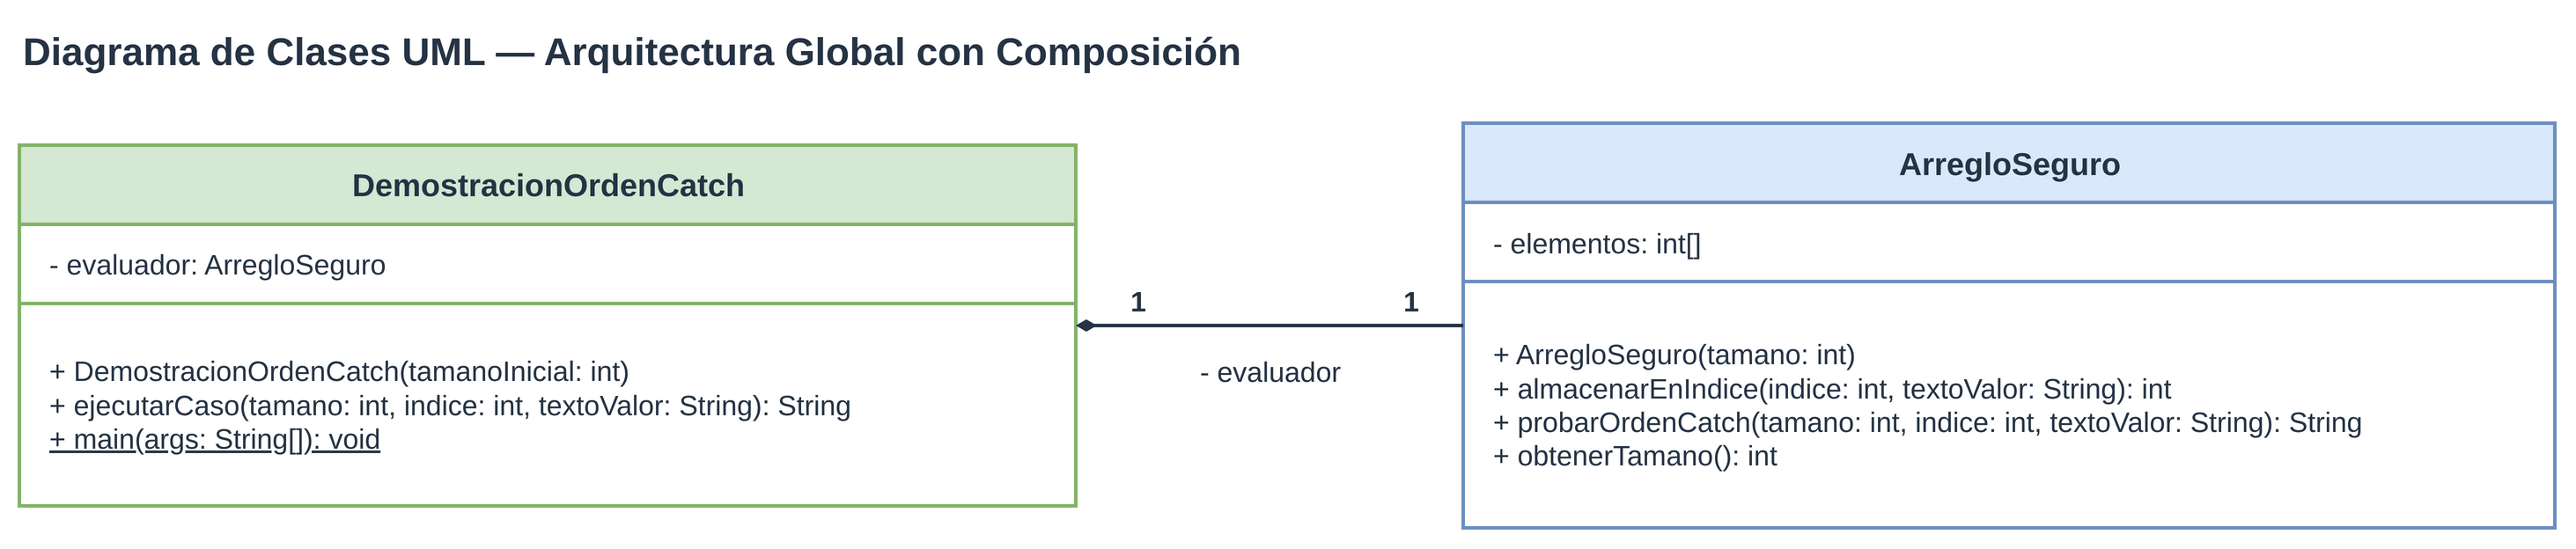
\includegraphics[width=\linewidth,height=0.68\textheight,keepaspectratio]{../Diagramas/uml_global.png}
    \end{column}
    \begin{column}{0.36\textwidth}
      \small
      \textbf{Decisiones de Diseño:}
      \begin{itemize}
        \item \textbf{Composición Fuerte ($1$ a $1$):} \texttt{DemostracionOrdenCatch} es propietaria exclusiva del objeto evaluador.
        \item \textbf{Ciclo de Vida Confinado:} La entidad evaluadora nace en el constructor del controlador y depende de su existencia.
        \item \textbf{Encapsulamiento:} Estado privado con interfaces públicas controladas.
      \end{itemize}
    \end{column}
  \end{columns}
\end{frame}

% Diapositiva 4: Diagrama de Clase ArregloSeguro
\begin{frame}{Diseño de la Entidad: Clase ArregloSeguro}
  \framesubtitle{Encapsulamiento del arreglo primitivo y evaluación de excepciones}
  \begin{columns}[c]
    \begin{column}{0.56\textwidth}
      \centering
      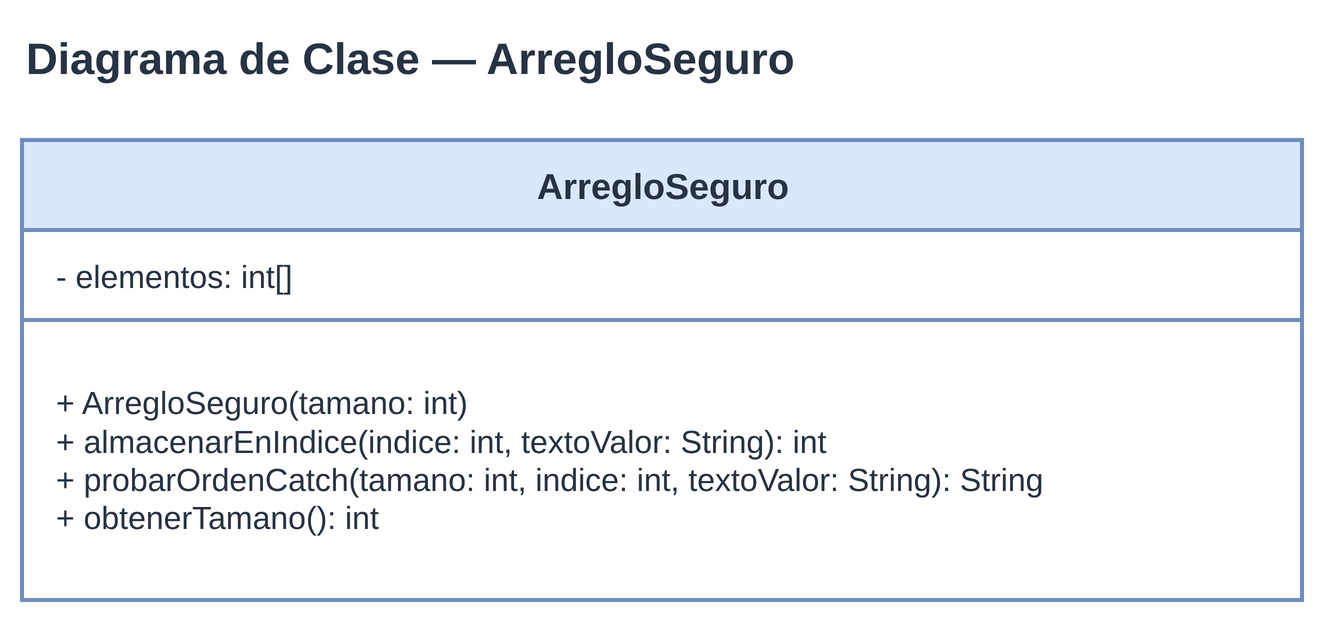
\includegraphics[width=\linewidth,height=0.68\textheight,keepaspectratio]{../Diagramas/uml_ArregloSeguro.png}
    \end{column}
    \begin{column}{0.44\textwidth}
      \small
      \textbf{Responsabilidades Clave:}
      \begin{itemize}
        \item \textbf{Encapsulamiento de Arreglo:} Protege el contenedor primitivo \texttt{elementos}.
        \item \textbf{Constructor Parametrizado:} Controla la dimensión e identifica tamaños ilícitos.
        \item \textbf{Inserción Controlada:} Convierte texto a valor primitivo y valida el índice destino.
        \item \textbf{Evaluador de Captura:} Orquesta la secuencia de bloques \texttt{catch} de lo específico a lo genérico.
      \end{itemize}
    \end{column}
  \end{columns}
\end{frame}

% Diapositiva 5: Diagrama de Clase DemostracionOrdenCatch
\begin{frame}{Diseño del Controlador: Clase DemostracionOrdenCatch}
  \framesubtitle{Coordinación del flujo interactivo y ejecución automatizada de pruebas}
  \begin{columns}[c]
    \begin{column}{0.56\textwidth}
      \centering
      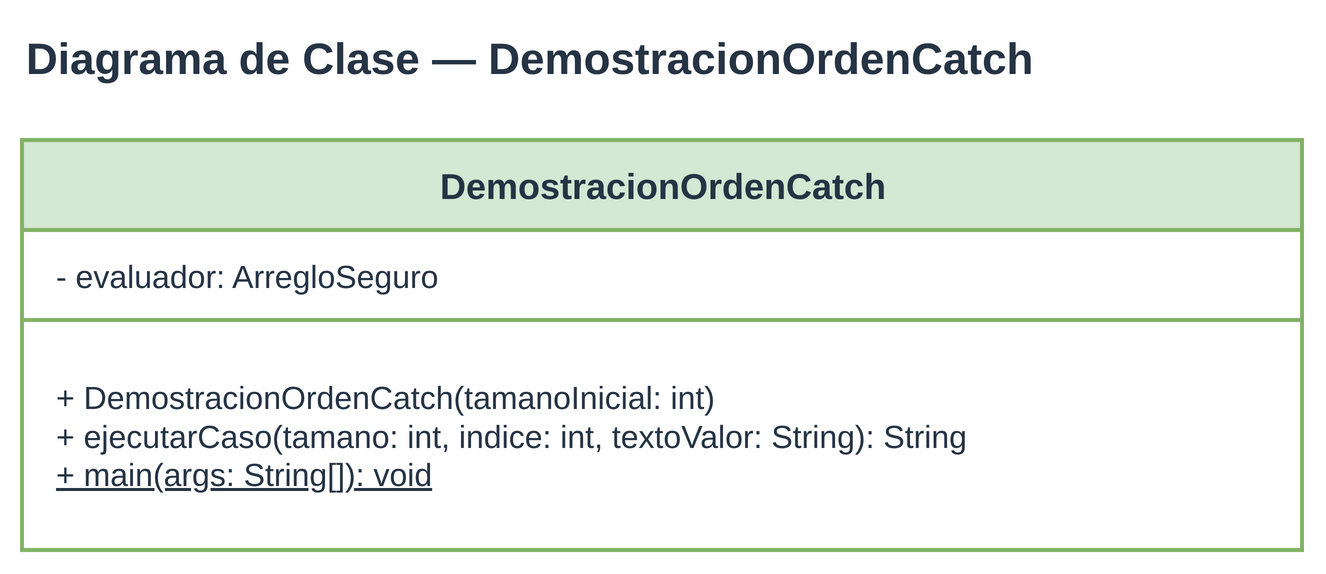
\includegraphics[width=\linewidth,height=0.68\textheight,keepaspectratio]{../Diagramas/uml_DemostracionOrdenCatch.png}
    \end{column}
    \begin{column}{0.44\textwidth}
      \small
      \textbf{Responsabilidades Clave:}
      \begin{itemize}
        \item \textbf{Punto de Entrada:} Método estático principal (\texttt{main}) para iniciar la ejecución.
        \item \textbf{Interacción por Consola:} Lectura guiada de tamaño, índice y valor de entrada.
        \item \textbf{Despacho de Casos:} Invoca al evaluador y formatea el reporte de salida.
        \item \textbf{Batería Automática:} Induce consecutivamente casos de índice, tamaño, formato y referencia.
      \end{itemize}
    \end{column}
  \end{columns}
\end{frame}

% Diapositiva 6: Flujo del Evaluador de Arreglo
\begin{frame}{Dinámica del Evaluador: Flujo de ArregloSeguro}
  \framesubtitle{Evaluación estructurada y secuencia ordenada de captura de excepciones}
  \begin{columns}[c]
    \begin{column}{0.52\textwidth}
      \centering
      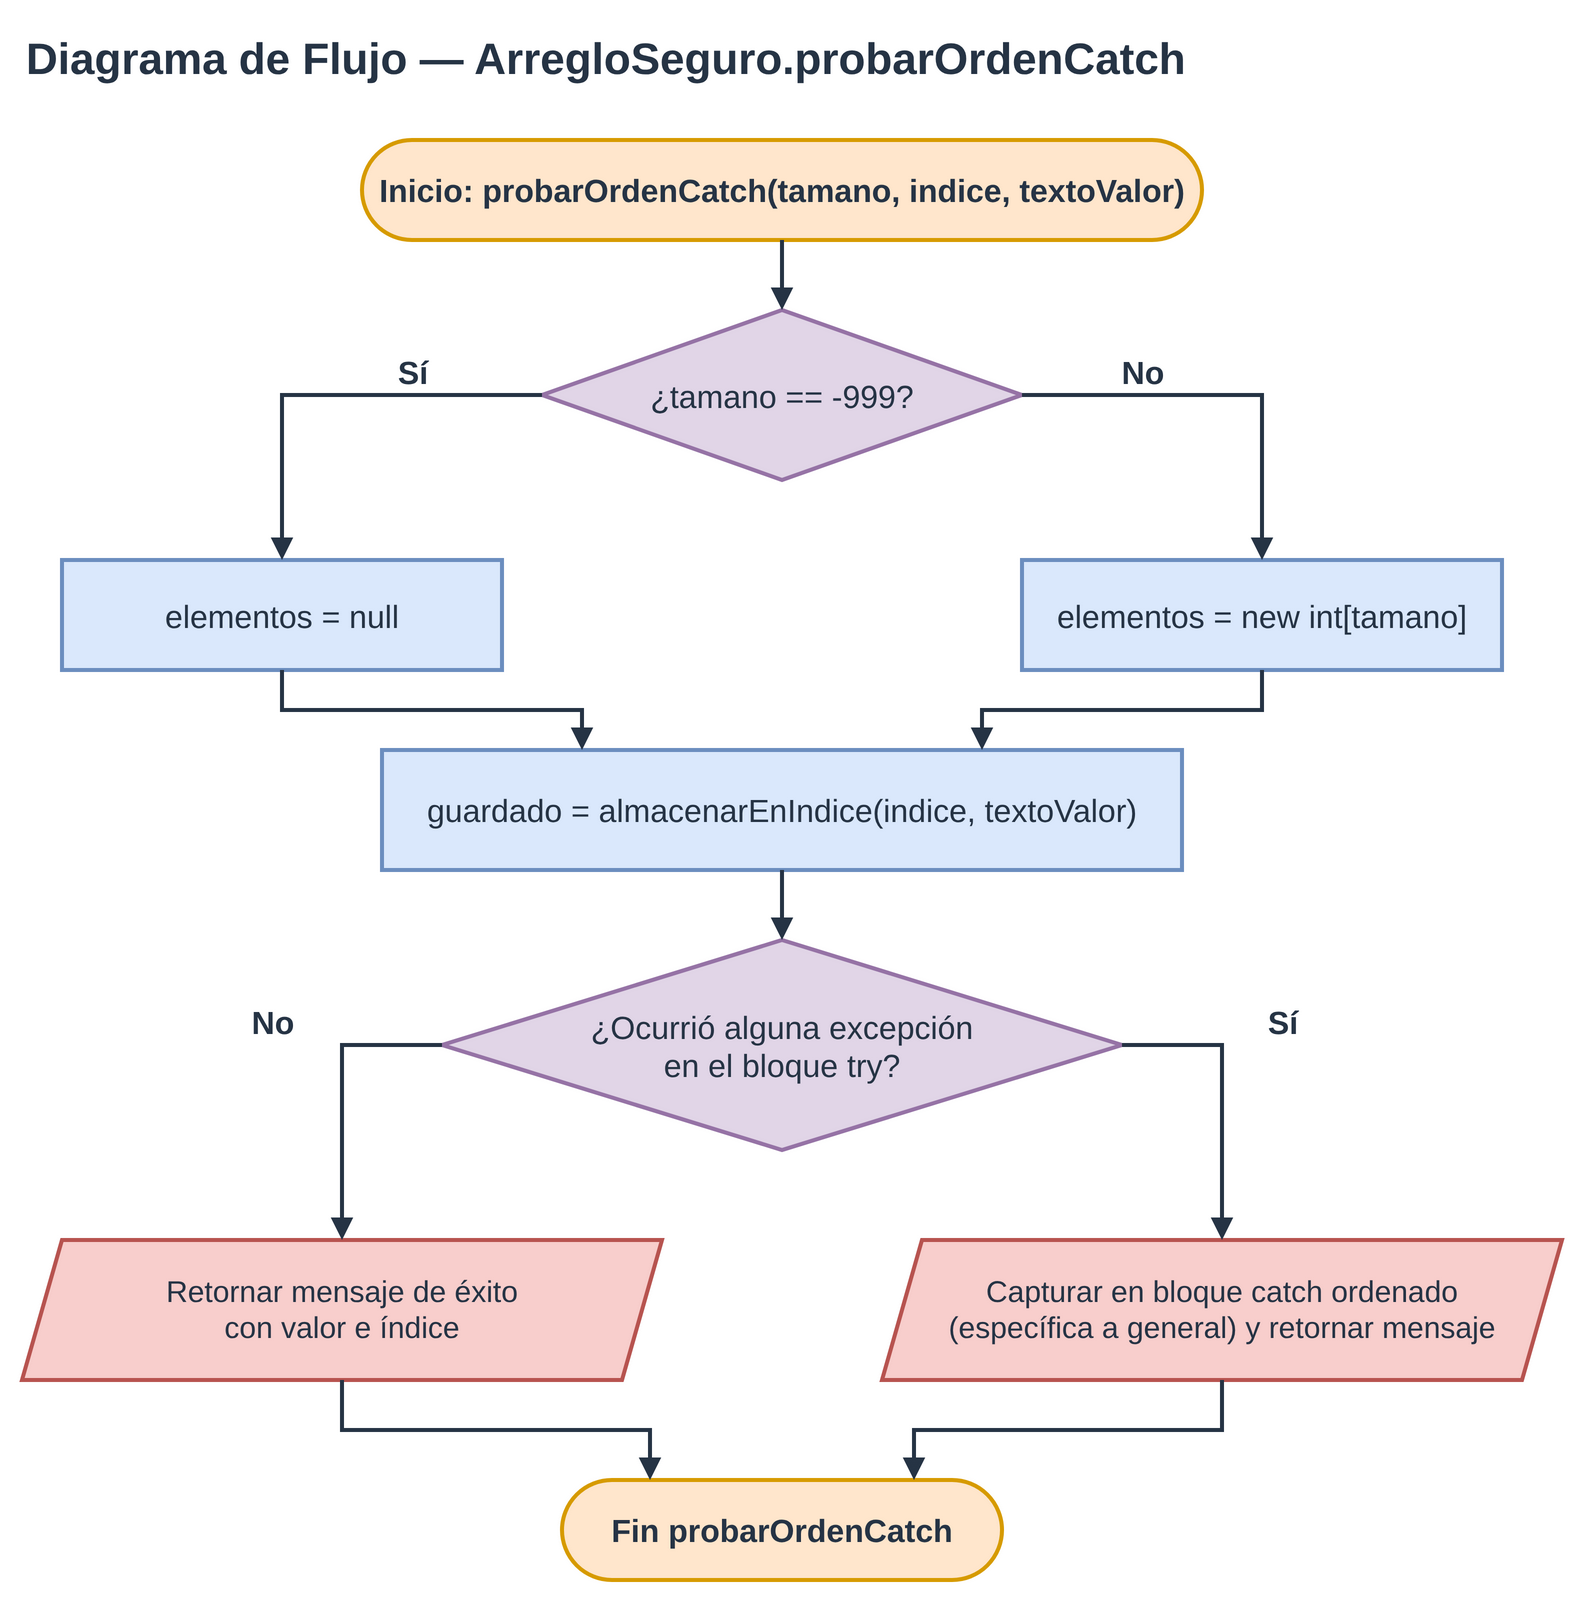
\includegraphics[width=\linewidth,height=0.72\textheight,keepaspectratio]{../Diagramas/flujo_ArregloSeguro.png}
    \end{column}
    \begin{column}{0.48\textwidth}
      \footnotesize
      \textbf{Secuencia de Decisiones:}
      \begin{itemize}
        \item \textbf{Inicialización:} Configura caso de referencia nula si el tamaño recibido es bandera.
        \item \textbf{Ejecución Segura:} Intenta reserva, conversión numérica e indexación.
        \item \textbf{Capturas Específicas Prioritarias:}
          \begin{enumerate}
            \item Índice fuera de rango (\texttt{ArrayIndexOutOfBounds})
            \item Tamaño negativo (\texttt{NegativeArraySize})
            \item Formato numérico (\texttt{NumberFormat})
            \item Referencia nula (\texttt{NullPointer})
          \end{enumerate}
        \item \textbf{Captura General:} Contención con clases base (\texttt{Exception}, \texttt{Throwable}) sin ocultar causas particulares.
      \end{itemize}
    \end{column}
  \end{columns}
\end{frame}

% Diapositiva 7: Flujo del Controlador Principal
\begin{frame}{Dinámica del Controlador: Flujo de DemostracionOrdenCatch}
  \framesubtitle{Lectura de parámetros por consola y ejecución secuencial de pruebas}
  \begin{columns}[c]
    \begin{column}{0.50\textwidth}
      \centering
      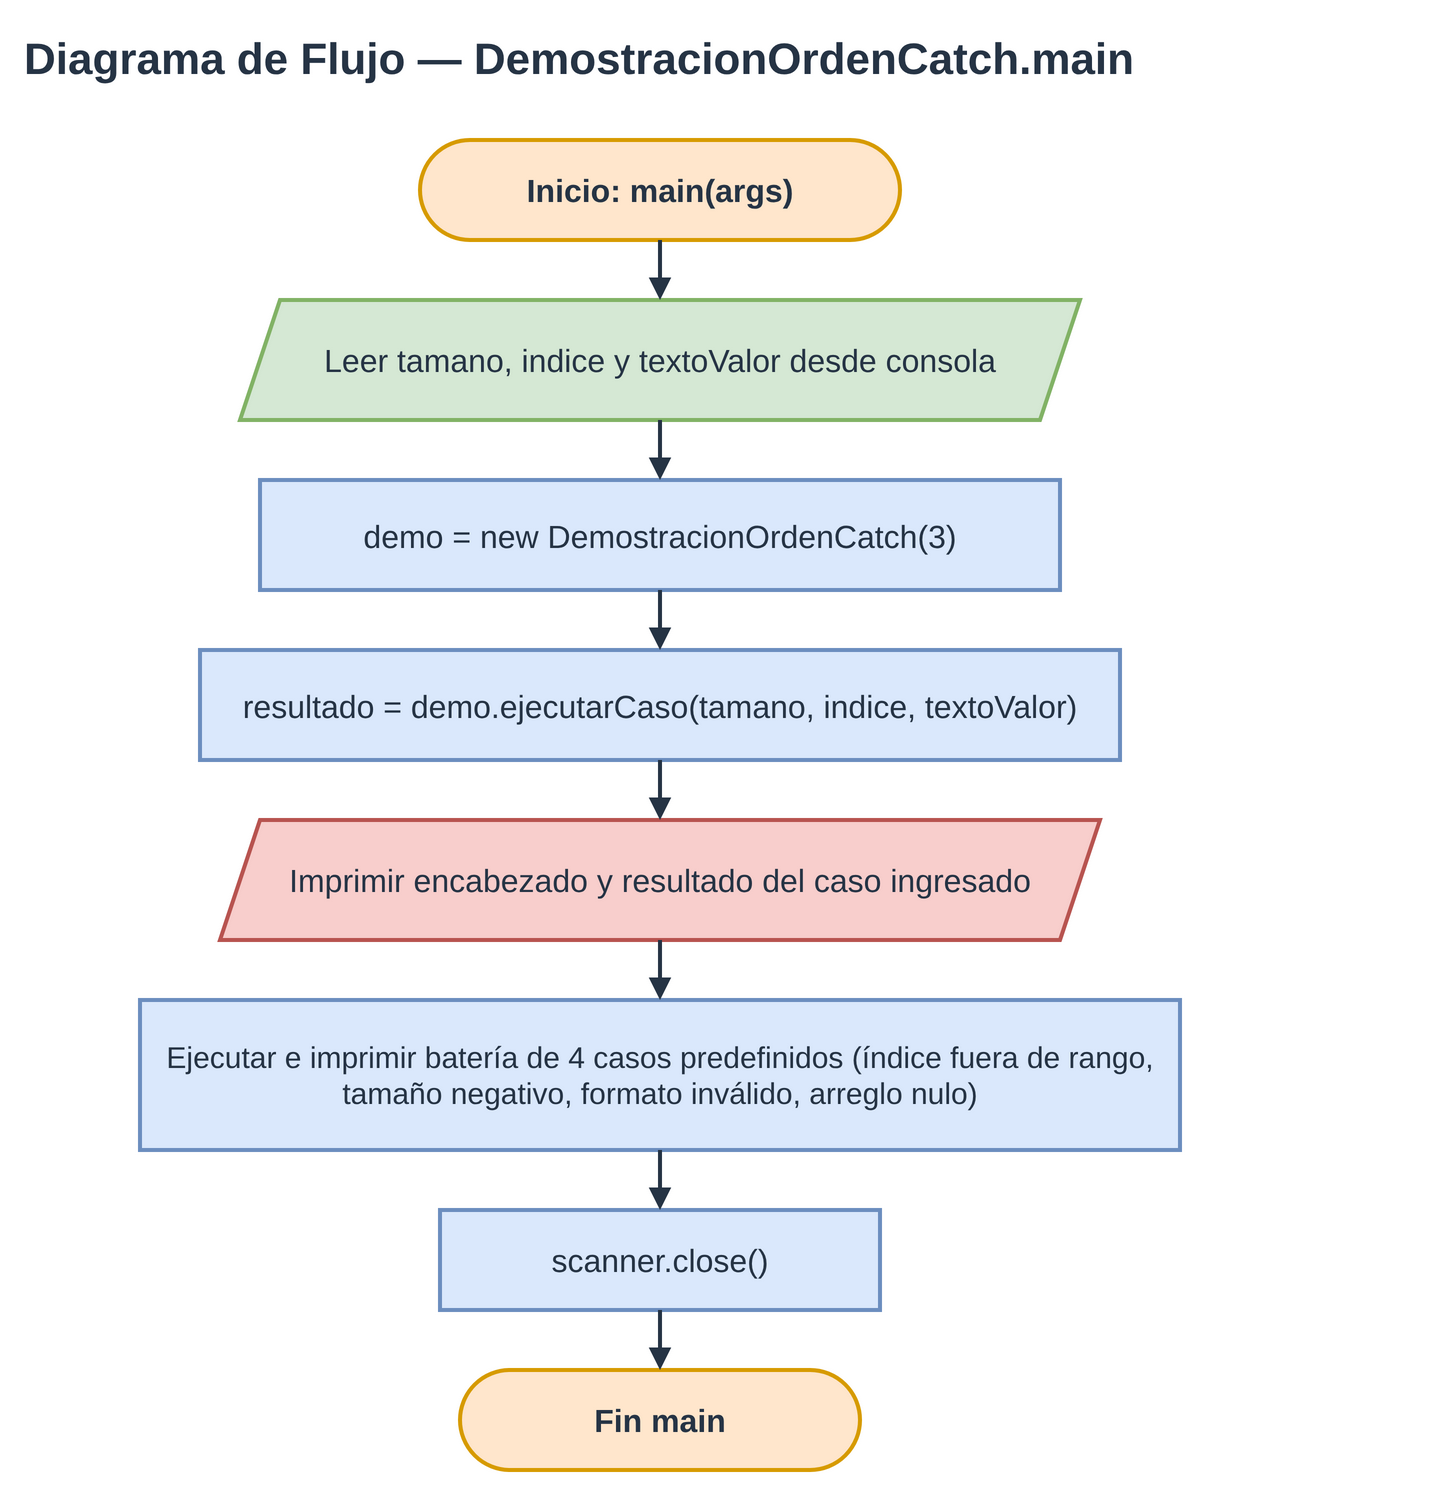
\includegraphics[width=\linewidth,height=0.72\textheight,keepaspectratio]{../Diagramas/flujo_DemostracionOrdenCatch.png}
    \end{column}
    \begin{column}{0.50\textwidth}
      \small
      \textbf{Secuencia Operativa:}
      \begin{itemize}
        \item \textbf{Inicialización:} Conexión a la consola y creación del controlador.
        \item \textbf{Caso de Usuario:} Lectura de parámetros dinámicos y envío al evaluador.
        \item \textbf{Batería de Pruebas Automáticas:}
          \begin{itemize}
            \item Índice desbordado.
            \item Dimensión negativa.
            \item Formato no convertible.
            \item Referencia no inicializada.
          \end{itemize}
        \item \textbf{Liberación:} Cierre de recursos de entrada y reporte en consola.
      \end{itemize}
    \end{column}
  \end{columns}
\end{frame}

% Diapositiva 8: Diagrama de Secuencia
\begin{frame}{Interacción Temporal: Diagrama de Secuencia}
  \framesubtitle{Colaboración entre actor, clase principal, instancia coordinadora y entidad evaluadora}
  \begin{columns}[c]
    \begin{column}{0.64\textwidth}
      \centering
      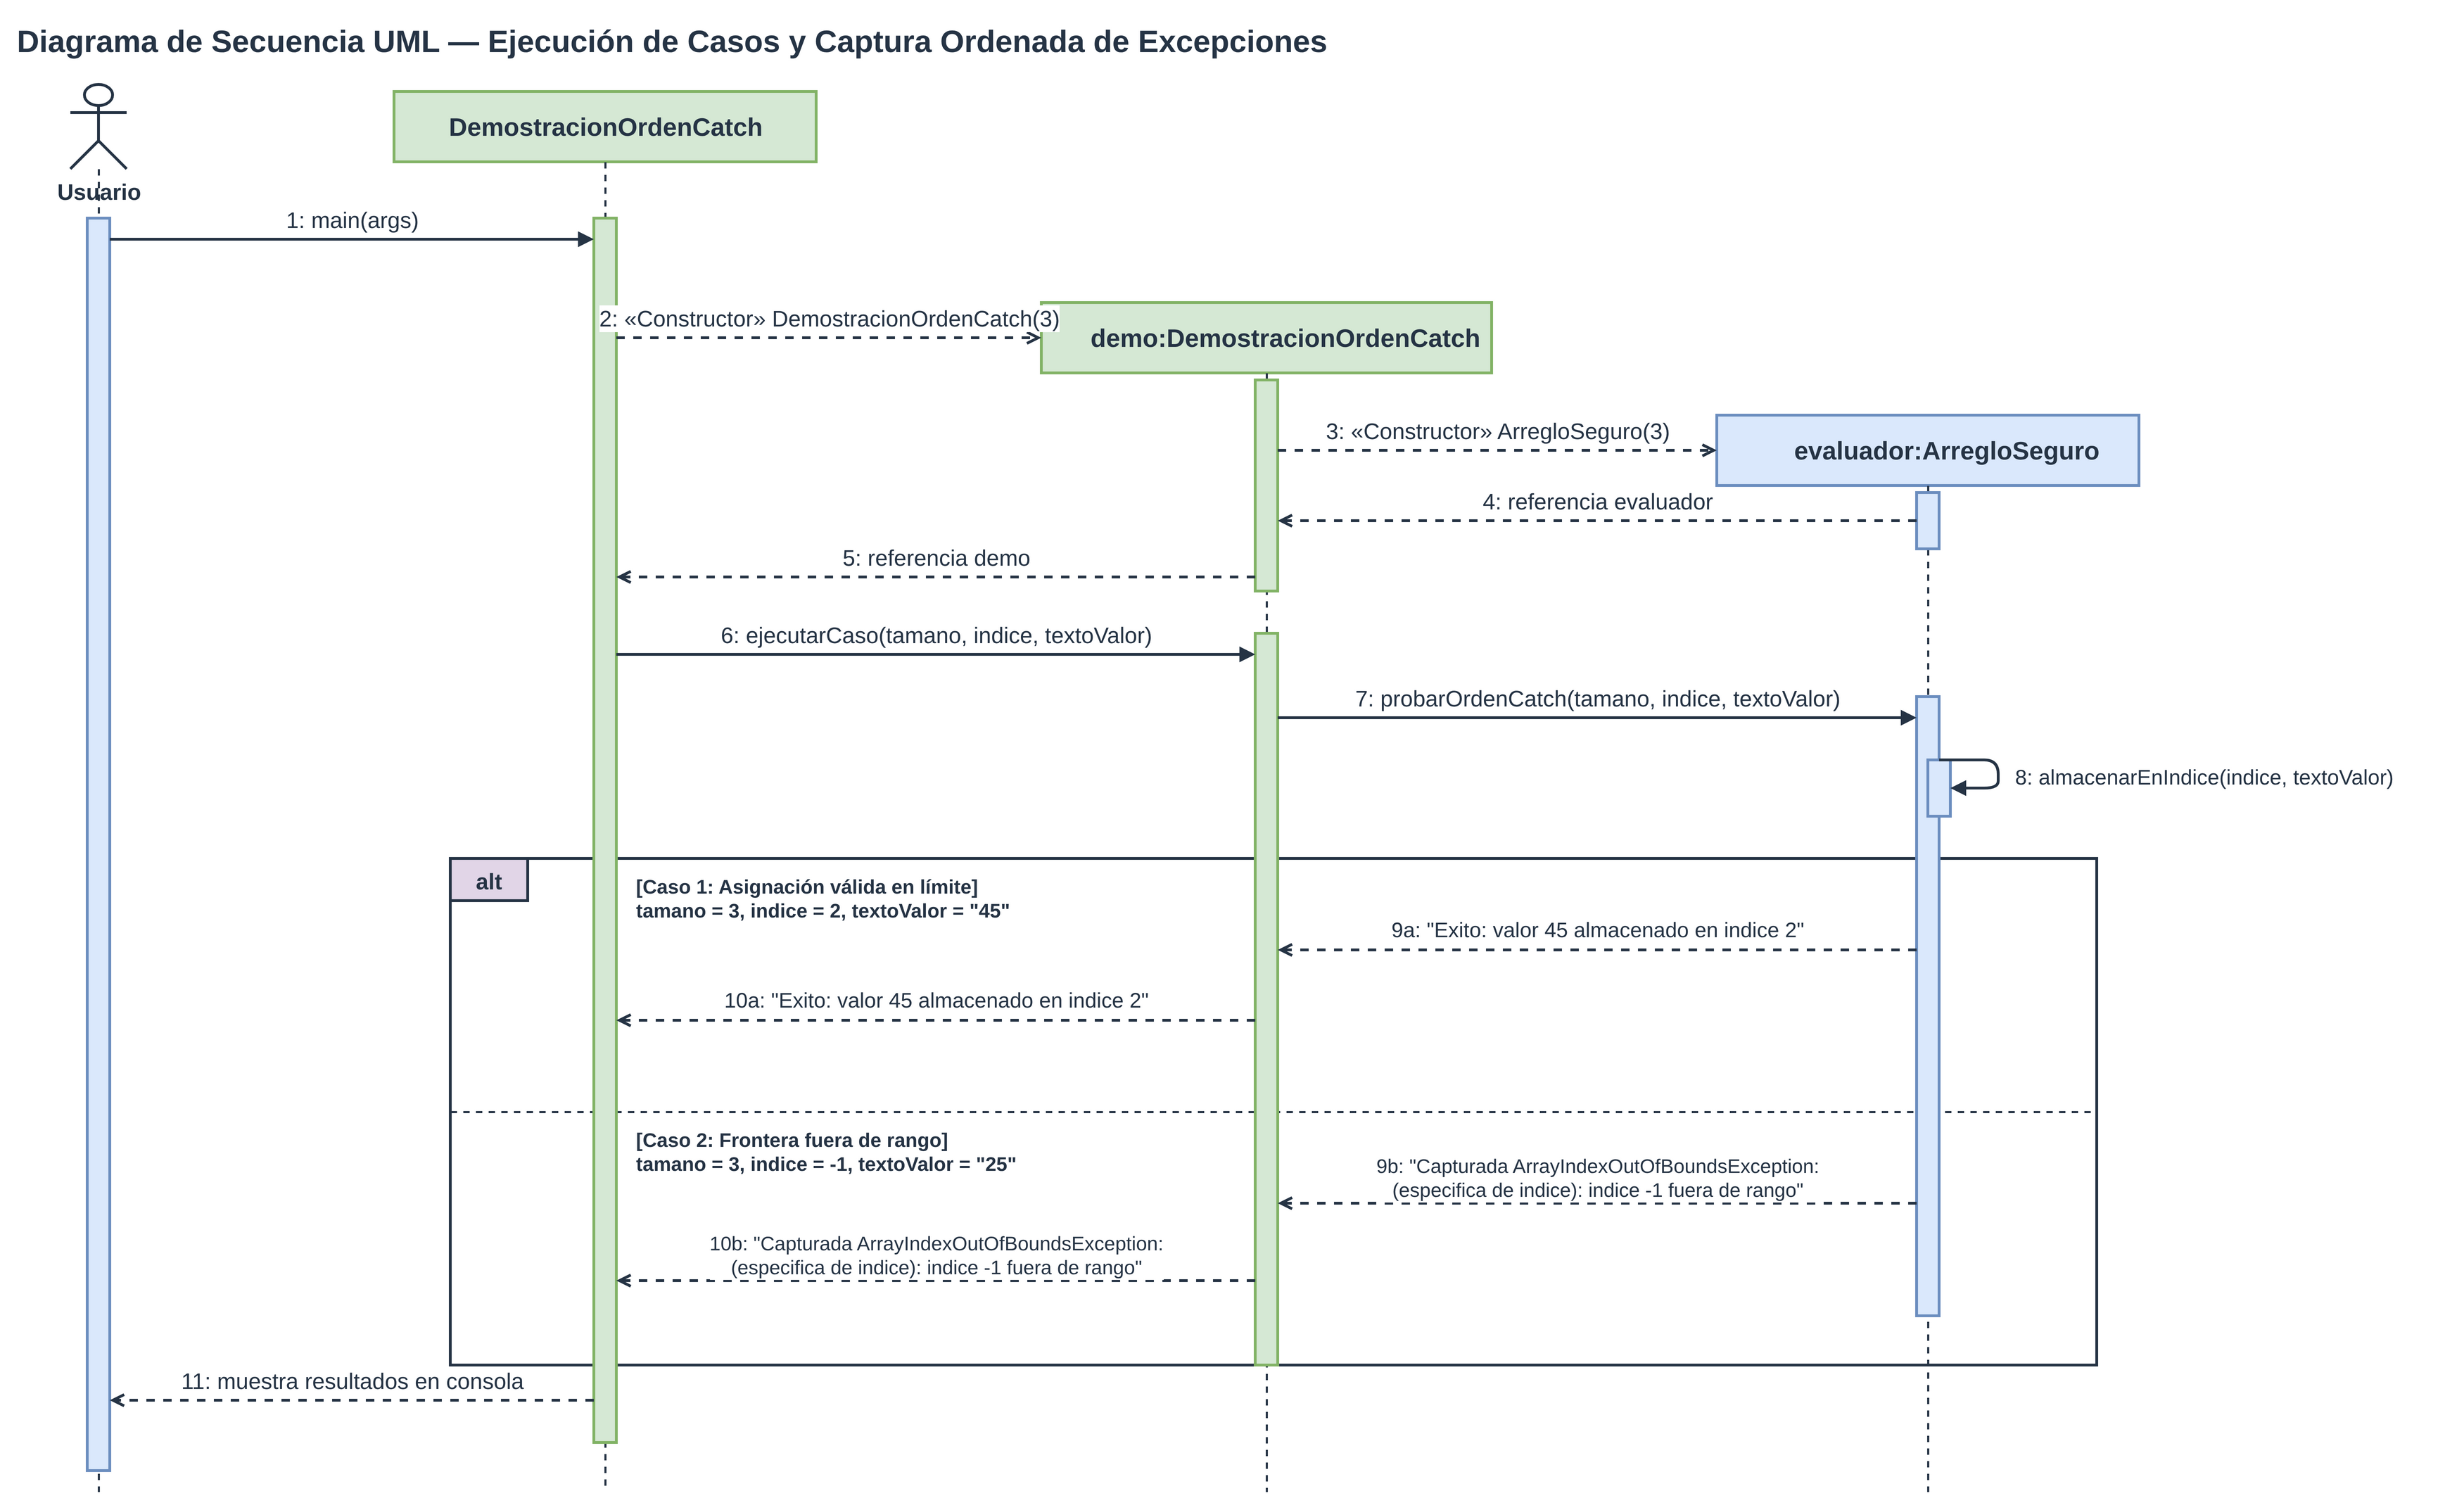
\includegraphics[width=\linewidth,height=0.70\textheight,keepaspectratio]{../Diagramas/secuencia_orden_catch.png}
    \end{column}
    \begin{column}{0.36\textwidth}
      \small
      \textbf{Secuencia de Mensajes:}
      \begin{itemize}
        \item \textbf{Arranque:} Invocación del método estático principal.
        \item \textbf{Composición:} Construcción de la instancia coordinadora y de la entidad de arreglo.
        \item \textbf{Delegación:} Envío de parámetros y autollamada anidada de inserción.
        \item \textbf{Bifurcación Alternativa:}
          \begin{itemize}
            \item \textbf{Caso 1:} Inserción exitosa.
            \item \textbf{Caso 2:} Captura unívoca por manejador específico de índice.
          \end{itemize}
      \end{itemize}
    \end{column}
  \end{columns}
\end{frame}

% Diapositiva 9: Conclusiones
\begin{frame}{Conclusiones y Principios de Diseño}
  \framesubtitle{Lecciones fundamentales de la gestión de excepciones en programación orientada a objetos}
  \begin{itemize}
    \item \textbf{Polimorfismo y Jerarquía:} La captura de excepciones responde rigurosamente al principio de sustitución de Liskov. El orden descendente de especificidad es indispensable para un manejo determinista y sin ambigüedades.
    \item \textbf{Diferenciación Arquitectónica:} Los fallos críticos de sistema (\texttt{Error}) deben segregarse categóricamente de las anomalías recuperables (\texttt{Exception}), asegurando la estabilidad del entorno de ejecución.
    \item \textbf{Robustez sobre Estructuras de Datos:} Las estructuras de almacenamiento indexadas exigen validación preventiva de invariantes combinada con bloques de contingencia tipados.
    \item \textbf{Diseño Profesional:} La anticipación de excepciones previene fallos silenciosos y garantiza la tolerancia a fallos tanto en servicios de cómputo como en interfaces gráficas interactivas.
  \end{itemize}
\end{frame}

\end{document}
